\documentclass[oneside,a4paper]{refart}
\usepackage[svgnames]{xcolor}
\usepackage{genogram}
\usepackage{rotating, mathabx, multirow}
\usepackage{cleveref}

\newcommand{\pn}{\texttt{genogram}} %package name
\newcommand{\key}[1]{\texttt{\textcolor{OrangeRed}{#1}}}
\newcommand{\kitem}[1]{\item[\key{#1}\texttt{=\textcolor{Purple}{<value>}}]} %key item
\newcommand{\command}[1]{\textcolor{Blue}{\texttt{\char`\\#1}}}
\newcommand{\citem}[1]{\item[\command{#1}]} %command item
\newcommand{\default}[1]{\textcolor{ForestGreen}{\ttfamily#1}}
\newcommand{\intextmarginnote}[2][2pt]{\hspace*{-\marginparwidth}\hspace*{-\marginparsep}#2\\[#1]}
\crefname{figure}{Figure}{Figures}
\crefname{section}{Section}{Sections}

\newcommand{\versionnumber}{1.0b}
\title{The \pn\ package: simply draw simple genograms}
\author{%
    \begin{tabular}{c}
        Alessandro Sciarra\\ {\small in progress}\\ \texttt{v\versionnumber}
    \end{tabular}
}

\date{}

\pagestyle{myheadings}
\markboth{The \pn\ package}%
         {The \pn\ package}

\makeindex

\setcounter{tocdepth}{2}
\settextfraction{0.85}

\begin{document}

\maketitle

%\vspace{-1cm}
\begin{abstract}
        This document is meant to be a short reference manual
        for the \pn\ package. \emph{Usage simplicity} is
        the main goal of the package and, hence, just knowing which
        commands are available should suffice for most of the users.
\end{abstract}

The \pn\ is the result of a simple need: To provide an interface (as simple as possible) between the complex world of \texttt{pgf/TikZ} and \LaTeX\ newbies, which know just the basics\footnote{Indeed, it has been also a good opportunity for the author to study and deepen into the \texttt{pgfkeys} world, but this is not so relevant.}.
An example of what can be produced with this package is probably a good starting point to have an idea about it.
The Reader is then encouraged to have a look to \cref{fig:genogram} at \cpageref{fig:genogram}, where commands used to draw the genogram have also been included.

\section{Package usage}

Although it is not at necessary, you might consider to use this package in combination with the \texttt{standalone} class.
The idea behind this choice would be to produce a genogram to be then possibly included as figure in another document.
A minimal, to-be-completed example might be the following.
\begin{verbatim}
    \documentclass[border=1mm]{standalone}
    \usepackage{genogram}

    \begin{document}
        \drawGenogram
    \end{document}
\end{verbatim}
In \cref{sec:code} you can find a way more complete example.

\section{Setting up and drawing the genogram}\label{sec:comm}

The flow to construct the genogram is simple.
At first, information about the family elements has to be provided and, only at the end, the resulting genogram has to be drawn.
In a more \TeX -nichal language, there is a drawing command to be issued at the end, after all other commands will have been used to set up features of the genogram.
As you will see the genogram is centred around a couple (husband and wife) and it is possible to draw their children, parents, siblings, brothers- and sisters-in-law, nephews and nieces.

\subsection*{Drawing rules to keep in mind}

Few rules exist and it is important to know them to achieve what desired.

\begin{itemize}
    \item In any couple, the man is always drawn left and the woman right.
    \item The order in which siblings are drawn is exactly as specified by the user
          This means that siblings of the husband specified before (after) the husband will be drawn left (right) of him.
          The same applies to the wife and her siblings.
    \item Children, nephews and nieces of the couple are as well drawn left to right respecting the order in which they were specified by the user.
\end{itemize}

\subsection*{The command keys}

All commands to set up the genogram have one optional value that consists of a comma separated list of \texttt{key=<value>} elements, where sometimes the \texttt{=<value>} is not needed and it must not be specified.
Possible keys, which will be mentioned later in the command description are the following.
\begin{description}
    \kitem{age} It is used to add the age of the person in the genogram.
    \kitem{name} It is used to add the name of the person in the genogram.
    \kitem{status} Possible values are \texttt{married}, \texttt{not married}, \texttt{separated} or \texttt{divorced}. This key determines how the couples in the genogram are connected.
    \kitem{of} Possible values are \texttt{wife} or \texttt{husband}. Use this key to specify who the command you are using refer to.
    \item[\key{dead}] It is used to specify that the command you are using refers to a dead person.
    \item[\key{male} or \key{female}] It is used to specify the sex of the element the command you are using refers to.
                                      Although they are available, there should normally be no need to use them, since any command has a default sex which is implied by the command name (e.g. the default sex of a sister is female.)
\end{description}

If you need to use for some reason a comma or an equal sign in the value of a key, you must enclose the value in curly braces, e.g. \verb|name={Paul, Jean}|.

\begin{center}\rule{0.5\textwidth}{1pt}\end{center}

\begingroup\small\marginlabel{\textcolor{DarkBlue}{\underline{\textsc{Advanced}}:}}
To offer to more advanced users the possibility to customise a bit more the genogram, two other keys are offered.
In order to use them, some \texttt{TikZ} knowledge is required.
Just ignore them, unless you need to do something that is not achievable using the provided commands.
In that case, these keys might be the way to go.

The two keys \key{extra node feature} and \key{extra label feature} accept as value a comma separated list of \texttt{key=<value>} elements which are forwarded to a \texttt{TikZ} node.
This implies that such a list has to be specified in curly braces, e.g.
\begin{center}
    \ttfamily extra node feature=\string{text=red, fill=yellow\string}
\end{center}
will make the genogram element text (the age) be typeset in red on yellow background.
As you might have already guessed, the genogram element (square or circle with inside the age) is a \texttt{TikZ} node to which the key \key{extra node feature} refers.
The name of a person in the genogram is also a \texttt{TikZ} node and you can customise it using the \key{extra label feature} key.
At the moment there is no key to customise paths.
\endgroup

\begin{center}\rule{0.5\textwidth}{1pt}\end{center}

\subsection*{The main commands}

Commands are in general used to add elements to the genogram.
Their names are self-explanatory and the following list provide the missing piece of information: Which key can be passed to which command.
Please, keep in mind that the default sex of each command is the one suggested by the command name.
However, just in case of special needs, all commands accept the \key{male} and \key{female} keys\footnote{Specifying the default sex is accepted, but it has no effect, unless the key is specified after having given the opposite sex key. Definitely a contrived scenario.}.

\begin{description}
    \advance\labelwidth by  1mm
    \advance\labelsep   by -1mm
    \citem{drawGenogram}
        This is probably the main command of the package, in the sense that it is responsible of drawing the genogram.
        Remember to use it only after having specified all family members, but do not forget to use it!
    \citem{wife[]}
        Accepted keys are \key{age}, \key{name}, \key{status} and \key{dead}.
    \citem{husband[]}
        Completely analogue to the \command{wife} command.
    \citem{daughter[]}
        Accepted keys are \key{age}, \key{name}, and \key{dead}.
        This command can and has to be repeated to specify more daughters.
    \citem{son[]}
        Completely analogue to the \command{daughter} command.
    \citem{mother[]}
        Accepted keys are \key{of}, \key{age}, \key{name}, \key{status} and \key{dead}.
        Use the \key{of} key to specify whether you are specifying the mother of the wife or of the husband.
    \citem{father[]}
        Completely analogue to the \command{mother} command.
    \citem{sister[]}
        Accepted keys are \key{of}, \key{age}, \key{name}, and \key{dead}.
        Use the \key{of} key to specify whether you are specifying a sister of the wife or of the husband.
        This command can and has to be repeated to specify more sisters.
    \citem{brother[]}
        Completely analogue to the \command{sister} command.
    \citem{sisterInLaw[]}
        Accepted keys are \key{of}, \key{age}, \key{name}, and \key{dead}.
        Use the \key{of} key to specify whether you are specifying a sister-in-law of the wife or of the husband.
        Pay attention to use this command in the right place, since it will refer to the last specified sibling (either of the wife or of the husband).
        It makes then sense to use this command after the \command{brother} command\footnote{The user might be confused since siblings of the husband (wife) are also siblings-in-law of the wife (husband). However, the \command{sisterInLaw} and \command{brotherInLaw} commands \textbf{cannot} be used to specify simple siblings. Use the \command{sister} and \command{brother} for that purpose.}.
    \citem{brotherInLaw[]}
        Completely analogue to the \command{sisterInLaw} command.
    \citem{niece[]}
        Accepted keys are \key{age}, \key{name}, and \key{dead}.
        This command can and has to be repeated to specify more nieces.
        Pay attention to use this command in the right place, since it will refer to the last specified sibling (either of the wife or of the husband).
        Note as well that this command will have no effect if the sister- or brother-in-law of the husband or of the wife has not been specified before.
        Said differently, the niece is drawn only if both her parents have been specified.
    \citem{nephew[]}
        Completely analogue to the \command{niece} command.
\end{description}

\paragraph{Remarks:}
\begin{itemize}
    \item The wife and the husband are always drawn.
    \item It is not possible to draw a single parent.
          Providing either the \command{mother} or the \command{father} command only will make a basic element for the unspecified parent be drawn.
    \item The \key{status} key needs to be specified only for one of the two elements of a couple.
          If you specify it in both elements, the later will be applied.
\end{itemize}

\subsection*{A command to customise the genogram appearance}

Although spacing between the genogram elements is treated in a quite dynamic way, it might be needed to affect the disposition of members in it.
For this purpose, you can use the \command{setBeforeDrawing[...]} command which also accepts a comma separated list of \texttt{key=<value>} as optional argument.
In this case the \texttt{<value>} is expected to be a length, i.e. a number followed by a unit of measure among \texttt{cm}, \texttt{mm}, \texttt{ex}, \texttt{em}, \texttt{in}, \texttt{pt}, \texttt{bp}, \texttt{dd} and \texttt{pc}\footnote{You can refer e.g. to \texttt{https://tex.stackexchange.com/a/8337/128737} for the conversions.}.
Possible keys are the following.

\intextmarginnote{\key{space around age}:}
This key refers to the white space around all ages in the genogram (between the number and either the square or the circle). The default value is \default{1pt}.

\intextmarginnote{\key{generation distance}:}
This is the \emph{vertical} distance between the centre of the shapes belonging to contiguous generations (e.g. the couple and the children). The default value is \default{3cm}.

\intextmarginnote{\key{couple distance}:}
This is the \emph{horizontal} distance between the centre of the husband and wife shapes. The default value is \default{10em} if the couple has less than 2 children, otherwise it is \default{5em} times the number of children.

\intextmarginnote{\key{husband parents distance}:}
This is the \emph{horizontal} distance between the centre of the husband parents shapes. The default value is \default{5em} times the number of the husband siblings increased by $1$.

\intextmarginnote{\key{wife parents distance}:}
This is the \emph{horizontal} distance between the centre of the wife parents shapes. The default value is \default{5em} times the number of the wife siblings increased by $1$.

\intextmarginnote{\key{broken couple symbol height}:}
For separated or divorced couple, you can change the height of the correspondent symbol using this key. The default value is \default{1ex}.

\intextmarginnote{\key{broken couple symbol width}:}
For separated or divorced couple, you can change the width of the correspondent symbol using this key. The default value is \default{0.5ex}.

\intextmarginnote{\key{children generation add distance below}:}
You might need to stretch or shrink the vertical line above each children; specify a positive or negative distance, respectively, which will be added to it. The default value is \default{0mm}.

\intextmarginnote{\key{siblings generation add distance above}:}
You might need to stretch or shrink the vertical line below each brother- or sister-in-law and their partners; specify a positive or negative distance, respectively, which will be added to it. The default value is \default{-3mm}.

\intextmarginnote{\key{siblings generation add distance below}:}
You might need to stretch or shrink the vertical line above each nephew and niece; specify a positive or negative distance, respectively, which will be added to it. The default value is \default{-3mm}.

\intextmarginnote{\key{husband people outer space}:}
This key may be used to change the \emph{horizontal} distance between the outermost people at the husband level (either the husband or his siblings) and the husband's parents. Brothers- or sisters-in-law are not considered here. Note that both negative or too-large-positive values are accepted, but they probably lead to an unwanted result. The default value is \default{2em}.

\intextmarginnote{\key{wife people outer space}:}
This key may be used to change the \emph{horizontal} distance between the outermost people at the wife level (either the wife or her siblings) and the wife's parents. Brothers- or sisters-in-law are not considered here. Note that both negative or too-large-positive values are accepted, but they probably lead to an unwanted result. The default value is \default{2em}.

\intextmarginnote{\key{niblings outer space}:}
This key may be used to change the \emph{horizontal} distance between the outermost niece(s) or nephew(s) and their parents. This key has no effect if only one nephew/niece is present. Note that both negative or too-large-positive values are accepted, but they probably lead to an unwanted result. The default value is \default{1em}.

\intextmarginnote{\key{children outer space}:}
This key may be used to change the \emph{horizontal} distance between the outermost children and their parents. This key has no effect is only one child is present. Note that both negative or too-large-positive values are accepted, but they probably lead to an unwanted result. The default value is \default{1em}.

\begin{center}\rule{0.5\textwidth}{1pt}\end{center}

\begingroup\small\marginlabel{\textcolor{DarkBlue}{\underline{\textsc{Advanced}}:}}
To offer to more advanced users the possibility to customise the \texttt{tikzpicture} even further, you can use the \command{addTikzGlobalOptions} command in order to specify global TikZ options.
For instance, use
\begin{center}
    \ttfamily\char`\\addTikzGlobalOptions\string{framed\string}
\end{center}
to add a frame to your genogram.
\endgroup

\begin{center}\rule{0.5\textwidth}{1pt}\end{center}

\section{The code to produce \cref{fig:genogram} {\scriptsize(without printing commands)}}\label{sec:code}

\marginlabel{\vspace{3.5mm} Black and white:}
\begin{verbatim}
  \documentclass[border=1mm]{standalone}
  \usepackage{genogram}

  \begin{document}
    \brother[of=husband, age=35, name=Bruce]
    \sisterInLaw[of=husband, age=32, name=Selina]
    \nephew[of=husband, age=9, name=Robin]
    \husband[name=Clark, age=30, status=not married]
    \sister[of=wife, age=36, name=Lucy]
    \wife[age=31, name=Lois]
    \son[age=7, name=Tony]
    \daughter[age=5, name=Pepper]
    \mother[of=wife, age=65, name=Ella]
    \father[of=wife, age=68, name=Sam]
    \mother[of=husband, dead, age=25, name=Lara]
    \father[of=husband, dead, age=32, name=Thomas, status=divorced]
    \setBeforeDrawing[husband parents distance=12em,
                      couple distance=20em, children outer space=6em,
                      siblings generation add distance below=-5mm]
    \addTikzGlobalOptions{framed}
    \drawGenogram
  \end{document}
\end{verbatim}
\begingroup\small


\newpage

\global\pdfpageattr\expandafter{\the\pdfpageattr/Rotate 90}
\begin{fullpage}
    \begin{sidewaysfigure}[ht]
        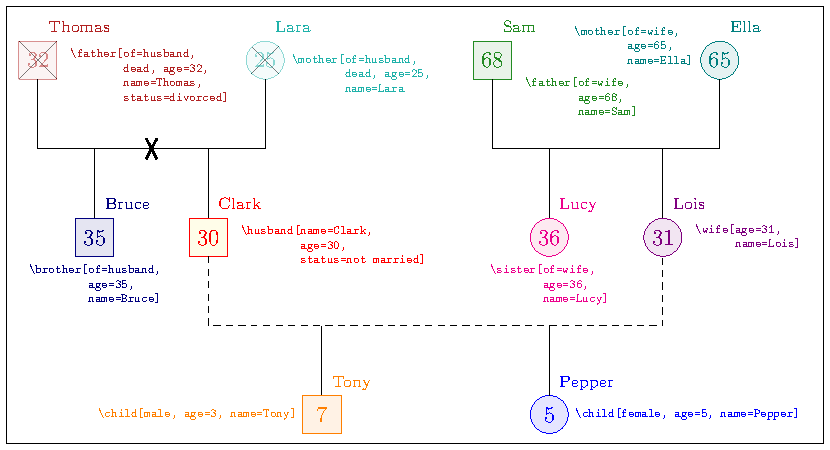
\includegraphics[width=\textwidth]{genogram_example}
        \caption{Demonstration of the \pn\ at work.}
        \label{fig:genogram}
    \end{sidewaysfigure}
\end{fullpage}
\global\pdfpageattr\expandafter{\the\pdfpageattr/Rotate 0}


\begingroup\small
\marginlabel{\vspace{3.6mm}Coloured version:}
\begin{verbatim}
  \documentclass[svgnames,border=1mm]{standalone}
  \usepackage{genogram}

  \begin{document}
    \brother[
        of=husband, age=35, name=Bruce,
        extra node feature={Navy, fill=Navy!10},
        extra label feature={text=Navy}]
    \sisterInLaw[
        of=husband, age=32, name=Selina,
        extra node feature={BlueViolet, fill=BlueViolet!10},
        extra label feature={text=BlueViolet}]
    \nephew[
        of=husband, age=9, name=Robin,
        extra node feature={OliveDrab, fill=OliveDrab!10},
        extra label feature={text=OliveDrab}]
    \husband[
        name=Clark, age=30, status=not married,
        extra node feature={red, fill=yellow!10},
        extra label feature={text=red}]
    \sister[
        of=wife, age=36, name=Lucy,
        extra node feature={magenta, fill=magenta!10},
        extra label feature={text=magenta}]
    \wife[
        age=31, name=Lois,
        extra node feature={violet, fill=violet!10},
        extra label feature={text=violet}]
    \son[
        age=7, name=Tony,
        extra node feature={orange, fill=orange!10},
        extra label feature={text=orange}]
    \daughter[
        age=5, name=Pepper,
        extra node feature={blue, fill=blue!10},
        extra label feature={text=blue}]
    \mother[
        of=wife, age=65, name=Ella,
        extra node feature={Teal, fill=Teal!10},
        extra label feature={text=Teal}]
    \father[
        of=wife, age=68, name=Sam,
        extra node feature={Goldenrod, fill=Goldenrod!10},
        extra label feature={text=Goldenrod}]
    \mother[
        of=husband, dead, age=25, name=Lara,
        extra node feature={LightSeaGreen, fill=LightSeaGreen!10},
        extra label feature={text=LightSeaGreen}]
    \father[
        of=husband, dead, age=32, name=Thomas, status=divorced,
        extra node feature={FireBrick, fill=FireBrick!10},
        extra label feature={text=FireBrick}]
    \setBeforeDrawing[
        husband parents distance=12em, couple distance=20em,
        siblings generation add distance below=-5mm,
        children outer space=6em]
    \addTikzGlobalOptions{framed}
    \drawGenogram
  \end{document}
\end{verbatim}

\endgroup


\section{Towards more freedom \hfill{\color{DarkBlue}\normalfont\scshape Advanced}}

If you know \LaTeX\ as well as \texttt{TikZ} more than just a bit, you might be interested in adding more details to your genogram.
The \command{addToTikzpicture\string{...\string}} command has been added exactly for you\footnote{Indeed, the commands in \cref{fig:genogram} have been added exactly using this command.}!
Specifying it -- clearly before \command{drawGenogram} -- you can continue drawing in the \texttt{tikzpicture} freely, after that the genogram has been drawn.
It is enough to give valid \texttt{TikZ} code in its mandatory argument.
Available \texttt{nodes} are
\begin{center}
    \ttfamily
    \begin{tabular}{l@{\hspace{4em}}l}
        gen@child<n> &\\
        gen@husband                      &  gen@wife                     \\
        gen@husband@mother               &  gen@wife@mother              \\
        gen@husband@father               &  gen@wife@father              \\
        gen@husband@sibling<n>           &  gen@wife@sibling<n>          \\
        gen@husband@sibling<n>@partner   &  gen@wife@sibling<n>@partner  \\
        gen@husband@sibling<n>@child<m>  &  gen@wife@sibling<n>@child<m> \\
    \end{tabular}
\end{center}
where the names as well as the positions should be self explanatory.
Note that \texttt{<n>} and \texttt{<m>} should be substituted with positive integers numbers and the index increases as the genogram elements are drawn\footnote{To be pedantic, the index does not increase at time of drawing and only nodes or coordinates are created in the \texttt{tikzpicture}. This should be irrelevant for you, though. The main message here is that the node indices respect the order in which genogram elements have been specified.}.
For each of the above listed nodes, two additional \texttt{coordinates} exists and they are called \texttt{<node name>@above} and \texttt{<node name>@below}.
These coordinates refer to points exactly at the line crossing point between generations.
You can use something like
\begin{verbatim}
    \addToTikzpicture{%
        \draw[red] (gen@husband@father@below) circle[radius=1pt];
    }
\end{verbatim}
to see where the coordinate \texttt{gen@husband@father@below} is.
\emph{If you know arrived here reading this section, you will know how to make use of this information.}



\end{document}
